\documentclass[]{article}
\usepackage{lmodern}
\usepackage{amssymb,amsmath}
\usepackage{ifxetex,ifluatex}
\usepackage{fixltx2e} % provides \textsubscript
\ifnum 0\ifxetex 1\fi\ifluatex 1\fi=0 % if pdftex
  \usepackage[T1]{fontenc}
  \usepackage[utf8]{inputenc}
\else % if luatex or xelatex
  \ifxetex
    \usepackage{mathspec}
  \else
    \usepackage{fontspec}
  \fi
  \defaultfontfeatures{Ligatures=TeX,Scale=MatchLowercase}
\fi
% use upquote if available, for straight quotes in verbatim environments
\IfFileExists{upquote.sty}{\usepackage{upquote}}{}
% use microtype if available
\IfFileExists{microtype.sty}{%
\usepackage{microtype}
\UseMicrotypeSet[protrusion]{basicmath} % disable protrusion for tt fonts
}{}
\usepackage[margin=1in]{geometry}
\usepackage{hyperref}
\hypersetup{unicode=true,
            pdftitle={Laborator 6},
            pdfborder={0 0 0},
            breaklinks=true}
\urlstyle{same}  % don't use monospace font for urls
\usepackage{color}
\usepackage{fancyvrb}
\newcommand{\VerbBar}{|}
\newcommand{\VERB}{\Verb[commandchars=\\\{\}]}
\DefineVerbatimEnvironment{Highlighting}{Verbatim}{commandchars=\\\{\}}
% Add ',fontsize=\small' for more characters per line
\usepackage{framed}
\definecolor{shadecolor}{RGB}{248,248,248}
\newenvironment{Shaded}{\begin{snugshade}}{\end{snugshade}}
\newcommand{\KeywordTok}[1]{\textcolor[rgb]{0.13,0.29,0.53}{\textbf{#1}}}
\newcommand{\DataTypeTok}[1]{\textcolor[rgb]{0.13,0.29,0.53}{#1}}
\newcommand{\DecValTok}[1]{\textcolor[rgb]{0.00,0.00,0.81}{#1}}
\newcommand{\BaseNTok}[1]{\textcolor[rgb]{0.00,0.00,0.81}{#1}}
\newcommand{\FloatTok}[1]{\textcolor[rgb]{0.00,0.00,0.81}{#1}}
\newcommand{\ConstantTok}[1]{\textcolor[rgb]{0.00,0.00,0.00}{#1}}
\newcommand{\CharTok}[1]{\textcolor[rgb]{0.31,0.60,0.02}{#1}}
\newcommand{\SpecialCharTok}[1]{\textcolor[rgb]{0.00,0.00,0.00}{#1}}
\newcommand{\StringTok}[1]{\textcolor[rgb]{0.31,0.60,0.02}{#1}}
\newcommand{\VerbatimStringTok}[1]{\textcolor[rgb]{0.31,0.60,0.02}{#1}}
\newcommand{\SpecialStringTok}[1]{\textcolor[rgb]{0.31,0.60,0.02}{#1}}
\newcommand{\ImportTok}[1]{#1}
\newcommand{\CommentTok}[1]{\textcolor[rgb]{0.56,0.35,0.01}{\textit{#1}}}
\newcommand{\DocumentationTok}[1]{\textcolor[rgb]{0.56,0.35,0.01}{\textbf{\textit{#1}}}}
\newcommand{\AnnotationTok}[1]{\textcolor[rgb]{0.56,0.35,0.01}{\textbf{\textit{#1}}}}
\newcommand{\CommentVarTok}[1]{\textcolor[rgb]{0.56,0.35,0.01}{\textbf{\textit{#1}}}}
\newcommand{\OtherTok}[1]{\textcolor[rgb]{0.56,0.35,0.01}{#1}}
\newcommand{\FunctionTok}[1]{\textcolor[rgb]{0.00,0.00,0.00}{#1}}
\newcommand{\VariableTok}[1]{\textcolor[rgb]{0.00,0.00,0.00}{#1}}
\newcommand{\ControlFlowTok}[1]{\textcolor[rgb]{0.13,0.29,0.53}{\textbf{#1}}}
\newcommand{\OperatorTok}[1]{\textcolor[rgb]{0.81,0.36,0.00}{\textbf{#1}}}
\newcommand{\BuiltInTok}[1]{#1}
\newcommand{\ExtensionTok}[1]{#1}
\newcommand{\PreprocessorTok}[1]{\textcolor[rgb]{0.56,0.35,0.01}{\textit{#1}}}
\newcommand{\AttributeTok}[1]{\textcolor[rgb]{0.77,0.63,0.00}{#1}}
\newcommand{\RegionMarkerTok}[1]{#1}
\newcommand{\InformationTok}[1]{\textcolor[rgb]{0.56,0.35,0.01}{\textbf{\textit{#1}}}}
\newcommand{\WarningTok}[1]{\textcolor[rgb]{0.56,0.35,0.01}{\textbf{\textit{#1}}}}
\newcommand{\AlertTok}[1]{\textcolor[rgb]{0.94,0.16,0.16}{#1}}
\newcommand{\ErrorTok}[1]{\textcolor[rgb]{0.64,0.00,0.00}{\textbf{#1}}}
\newcommand{\NormalTok}[1]{#1}
\usepackage{graphicx,grffile}
\makeatletter
\def\maxwidth{\ifdim\Gin@nat@width>\linewidth\linewidth\else\Gin@nat@width\fi}
\def\maxheight{\ifdim\Gin@nat@height>\textheight\textheight\else\Gin@nat@height\fi}
\makeatother
% Scale images if necessary, so that they will not overflow the page
% margins by default, and it is still possible to overwrite the defaults
% using explicit options in \includegraphics[width, height, ...]{}
\setkeys{Gin}{width=\maxwidth,height=\maxheight,keepaspectratio}
\IfFileExists{parskip.sty}{%
\usepackage{parskip}
}{% else
\setlength{\parindent}{0pt}
\setlength{\parskip}{6pt plus 2pt minus 1pt}
}
\setlength{\emergencystretch}{3em}  % prevent overfull lines
\providecommand{\tightlist}{%
  \setlength{\itemsep}{0pt}\setlength{\parskip}{0pt}}
\setcounter{secnumdepth}{5}
% Redefines (sub)paragraphs to behave more like sections
\ifx\paragraph\undefined\else
\let\oldparagraph\paragraph
\renewcommand{\paragraph}[1]{\oldparagraph{#1}\mbox{}}
\fi
\ifx\subparagraph\undefined\else
\let\oldsubparagraph\subparagraph
\renewcommand{\subparagraph}[1]{\oldsubparagraph{#1}\mbox{}}
\fi

%%% Use protect on footnotes to avoid problems with footnotes in titles
\let\rmarkdownfootnote\footnote%
\def\footnote{\protect\rmarkdownfootnote}

%%% Change title format to be more compact
\usepackage{titling}

% Create subtitle command for use in maketitle
\newcommand{\subtitle}[1]{
  \posttitle{
    \begin{center}\large#1\end{center}
    }
}

\setlength{\droptitle}{-2em}
  \title{Laborator 6}
  \pretitle{\vspace{\droptitle}\centering\huge}
  \posttitle{\par}
\subtitle{Proprietăți ale estimatorilor}
  \author{}
  \preauthor{}\postauthor{}
  \date{}
  \predate{}\postdate{}

\usepackage{booktabs}
\usepackage{longtable}
\usepackage{framed,color}
\definecolor{shadecolor}{RGB}{248, 248, 248}
\definecolor{shadecolor1}{RGB}{216,225,235}
\definecolor{framecolor}{RGB}{108,123,13}

\ifxetex
  \usepackage{letltxmacro}
  \setlength{\XeTeXLinkMargin}{1pt}
  \LetLtxMacro\SavedIncludeGraphics\includegraphics
  \def\includegraphics#1#{% #1 catches optional stuff (star/opt. arg.)
    \IncludeGraphicsAux{#1}%
  }%
  \newcommand*{\IncludeGraphicsAux}[2]{%
    \XeTeXLinkBox{%
      \SavedIncludeGraphics#1{#2}%
    }%
  }%
\fi

\newenvironment{frshaded*}{%
  \def\FrameCommand{\fboxrule=\FrameRule\fboxsep=\FrameSep \fcolorbox{framecolor}{shadecolor1}}%
  \MakeFramed {\advance\hsize-\width \FrameRestore}}%
{\endMakeFramed}

\newenvironment{rmdblock}[1]
  {\begin{frshaded*}
  \begin{itemize}
  \renewcommand{\labelitemi}{
    \raisebox{-.7\height}[0pt][0pt]{
      {\setkeys{Gin}{width=2em,keepaspectratio}\includegraphics{images/icons/#1}}
    }
  }
  \item
  }
  {
  \end{itemize}
  \end{frshaded*}
  }
  
\newenvironment{rmdcaution}
  {\begin{rmdblock}{caution}}
  {\end{rmdblock}}
% \newenvironment{rmdinsight}
%   {\begin{rmdblock}{insight}}
%   {\end{rmdblock}}
\newenvironment{rmdexercise}
  {\begin{rmdblock}{exercise}}
  {\end{rmdblock}}
\newenvironment{rmdtip}
  {\begin{rmdblock}{tip}}
  {\end{rmdblock}}
  
  
%%%%%%%%%%%%%%%%%%%%%%%%%%%%%%%%%%%%%%%%%%%%%%%%%%%%%%%%%%%%%%%%%%%%%%%%%%%%%%%%%%%%%%%%%%%%%%%%%%%%%%%%%%%%%%%%%%%%%
%%%%%%%%%%% For insight block %%%%%%%%%%%%%%%%%%%%%%%%%%
\definecolor{shadecolor_insight}{RGB}{223,240,216}
\definecolor{framecolor_insight}{RGB}{136,193,137}

\newenvironment{frshaded_insight*}{%
  \def\FrameCommand{\fboxrule=\FrameRule\fboxsep=\FrameSep \fcolorbox{framecolor_insight}{shadecolor_insight}}%
  \MakeFramed {\advance\hsize-\width \FrameRestore}}%
{\endMakeFramed}

\newenvironment{rmdblock_insight}[1]
  {\begin{frshaded_insight*}
  \begin{itemize}
  \renewcommand{\labelitemi}{
    \raisebox{-.7\height}[0pt][0pt]{
      {\setkeys{Gin}{width=2em,keepaspectratio}\includegraphics{images/icons/#1}}
    }
  }
  \item
  }
  {
  \end{itemize}
  \end{frshaded_insight*}
  }
  
\newenvironment{rmdinsight}
  {\begin{rmdblock_insight}{insight}}
  {\end{rmdblock_insight}}
  
%%%%%%%%%%%%%%%%%%%%%%%%%%%%%%%%%%%%%%%%%%%%%%%%%%%%%%%%%%%%%%%%%%%%%%%%%%%%%%%%%%%%%%%%%%%%%%%%%%%%%%%%%%%%%%%%%%%%%
\usepackage{subfigure}
\usepackage{booktabs}
\usepackage{slashbox}
\usepackage{color}
%%%%%%%%%%%%%%%%%%%%%%%%%%%%%%%%%%%%%%%%%%%%%%%%%%%%%%%%%%%%%%%%%%%%%%%%%%%%%%%%%%%%%%%%%%%%%%%%%%%%%%%%%%%%%%%%%%%%%
%CITEVA DEFINITII
\def\om{\omega}
\def\Om{\Omega}
\def\et{\eta}
\def\td{\tilde{\delta}}
\def\m{{\mu}}
\def\n{{\nu}}
\def\k{{\kappa}}
\def\l{{\lambda}}
\def\L{{\Lambda}}
\def\g{{\gamma}}
\def\a{{\alpha}}
\def\e{{\varepsilon}}
\def\b{{\beta}}
\def\G{{\Gamma}}
\def\d{{\delta}}
\def\D{{\Delta}}
\def\t{{\theta}}
\def\s{{\sigma}}
\def\S{{\Sigma}}
\def\z{{\zeta}}
\def\qed{\hfill\Box}
\def\ds{\displaystyle}
\def\mc{\mathcal}
%%%%%%%%%%%%%%%%%%%%%%%%%%%%%%%%%%%%%%%%%%%%%%%%%%%%%%%%%%%%%%%%%%%%%%%%%%%%%%%%%%%%%%%%%%%%%%%%%%%%%%%%%%%%%%%%%%%%%%
\def\1{{\mathbf 1}}
\def\CC{{\mathbb C}}
\def\VV{{\mathbb V}}
\def\RR{{\mathbb R}}
\def\QQ{{\mathbb Q}}
\def\ZZ{{\mathbb Z}}
\def\PP{{\mathbb P}}
\def\EE{{\mathbb E}}
\def\NN{{\mathbb N}}
\def\FF{{\mathbb F}}
%\def\SS{{\mathbb S}}
\def\MA{{\mathcal A}}
\def\MO{{\mathcal O}}
\def\MF{{\mathcal F}}
\def\ME{{\mathcal E}}
\def\MR{{\mathcal R}}
\def\MB{{\mathcal B}}
\def\MM{{\mathcal M}}
\def\MN{{\mathcal N}}
\def\MU{{\mathcal U}}
\def\MP{{\mathcal P}}
\def\MS{{\mathcal S}}
\def\MBS{{\mathbf S}}
\def\MX{{\bm{ \mathscr X}}}

% independent sign
\newcommand\independent{\protect\mathpalette{\protect\independenT}{\perp}}
\def\independenT#1#2{\mathrel{\rlap{$#1#2$}\mkern2mu{#1#2}}}

\renewcommand{\figurename}{Fig.}

%%%%%%%%%%%%%%%%%%%%%%%%%%%%%%%%%%%%%%%%%%%%%%%%%%%%%%%%%%%%%%%%%%%%%%%%%%%%%%%%%%%%%%%%%%%%%%%%%%%%%%%%%%%%%%%%%%%%%
%Header and Footer
\usepackage{fancyhdr}

\pagestyle{fancy}
\fancyhf{}
\rhead{Universitatea din Bucure\c sti\\ Facultatea de Matematic\u a \c si Informatic\u a}
\lhead{\textit{Curs}: Statistic\u a\\ \textit{Instructori}: A. Am\u arioarei, S. Cojocea}
\rfoot{Pagina \thepage}
\lfoot{Grupele: 301, 311, 321}
%%%%%%%%%%%%%%%%%%%%%%%%%%%%%%%%%%%%%%%

\begin{document}
\maketitle

%%%%%%%%%%%%%%%%%%%%%%%%
\thispagestyle{fancy}

Obiectivul acestui laborator este de a ilustra noțiunea de consistență a
unui estimator precum și de a compara mai mulți estimatori.

\section{Exemplu de comparare a trei
estimatori}\label{exemplu-de-comparare-a-trei-estimatori}

\begin{rmdexercise}
Fie \(X_1,X_2,\ldots,X_n\) un eșantion de talie \(n\) dintr-o populație
normală de medie \(\mu\) și varianță \(\sigma^2\). Atunci

\[
  \hat{\mu}_1 = \frac{1}{n}\sum_{i=1}^{n}X_i, \quad \hat{\mu}_2 = M_n\,(\text{mediana}\,), \quad \hat{\mu}_3 = \frac{X_{(1)} + X_{(n)}}{2}
\]

sunt trei estimatori punctuali pentru \(\mu\). Creați o funcție care să
ilustreze cum sunt repartizați cei trei estimatori. Începeți cu
\(n = 10\), \(\mu = 0\) și \(\sigma^2 = 1\) și trasați histogramele
pentru a-i compara. Ce se întâmplă dacă schimbați \(n\), \(\mu\) sau
\(\sigma^2\) ?
\end{rmdexercise}

Vom crea o funcție numită \texttt{norm\_estimators} care va construi
repartițiile celor trei estimatori:

\begin{Shaded}
\begin{Highlighting}[]
\NormalTok{norm_estimators =}\StringTok{ }\ControlFlowTok{function}\NormalTok{(n, mu, sigma, S)\{}
  \CommentTok{# Initializam}
\NormalTok{  mu1 =}\StringTok{ }\KeywordTok{numeric}\NormalTok{(S)}
\NormalTok{  mu2 =}\StringTok{ }\KeywordTok{numeric}\NormalTok{(S)}
\NormalTok{  mu3 =}\StringTok{ }\KeywordTok{numeric}\NormalTok{(S)}
  
  \CommentTok{# repetam experimentul de S ori}
  \ControlFlowTok{for}\NormalTok{ (i }\ControlFlowTok{in} \DecValTok{1}\OperatorTok{:}\NormalTok{S)\{}
\NormalTok{    x =}\StringTok{ }\KeywordTok{rnorm}\NormalTok{(n, }\DataTypeTok{mean =}\NormalTok{ mu, }\DataTypeTok{sd =}\NormalTok{ sigma)}
    
    \CommentTok{# calculam estimatorii}
\NormalTok{    mu1[i] =}\StringTok{ }\KeywordTok{mean}\NormalTok{(x)}
\NormalTok{    mu2[i] =}\StringTok{ }\KeywordTok{median}\NormalTok{(x)}
\NormalTok{    mu3[i] =}\StringTok{ }\NormalTok{(}\KeywordTok{min}\NormalTok{(x)}\OperatorTok{+}\KeywordTok{max}\NormalTok{(x))}\OperatorTok{/}\DecValTok{2}
\NormalTok{  \}}
  
  \CommentTok{# afisam variantele estimatorilor }
  \KeywordTok{print}\NormalTok{(}\KeywordTok{cbind}\NormalTok{(}\DataTypeTok{var_mu1 =} \KeywordTok{var}\NormalTok{(mu1), }\DataTypeTok{var_mu2 =} \KeywordTok{var}\NormalTok{(mu2), }\DataTypeTok{var_mu3 =} \KeywordTok{var}\NormalTok{(mu3)))}
  
 \KeywordTok{return}\NormalTok{(}\KeywordTok{cbind}\NormalTok{(}\DataTypeTok{mu1 =}\NormalTok{ mu1, }\DataTypeTok{mu2 =}\NormalTok{ mu2, }\DataTypeTok{mu3 =}\NormalTok{ mu3))}
  
\NormalTok{\}}
\end{Highlighting}
\end{Shaded}

Pentru a ilustra grafic histogramele celor trei estimatori, considerăm
\(\mu = 0\) și \(\sigma^2 = 1\) și avem:

\begin{verbatim}
          var_mu1     var_mu2    var_mu3
[1,] 0.0009932978 0.001566703 0.06160938
\end{verbatim}

\begin{center}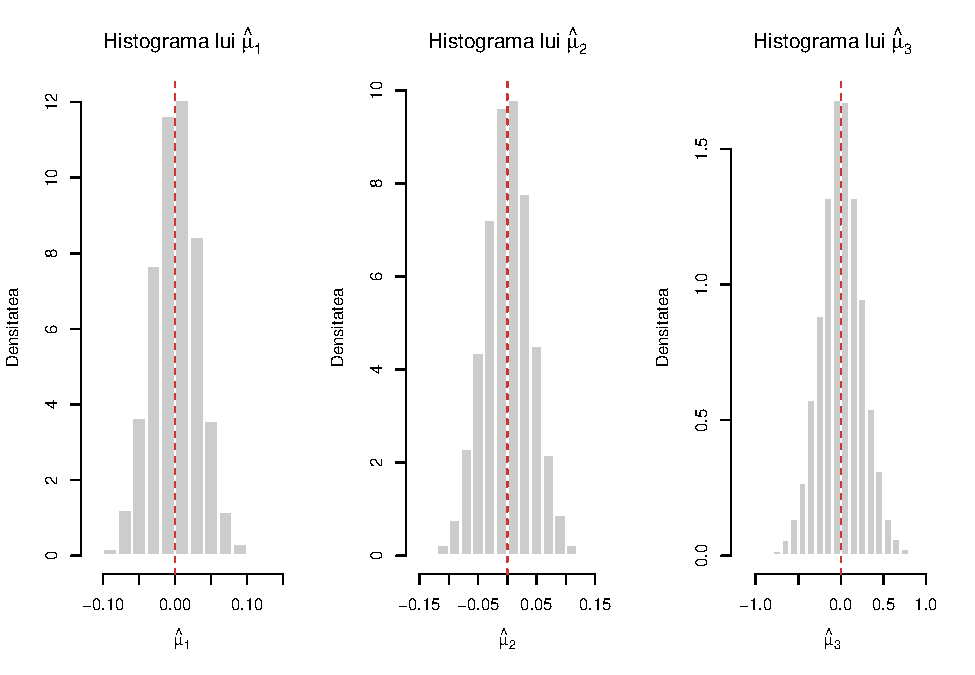
\includegraphics[width=0.7\linewidth]{Lab_6_files/figure-latex/unnamed-chunk-4-1} \end{center}

\section{Ilustrarea consistenței unui
estimator}\label{ilustrarea-consistentei-unui-estimator}

\begin{rmdexercise}
Fie \(X_1,X_2,\ldots,X_n\) un eșantion de talie \(n\) dintr-o populație
\(Pois(\theta)\). Ilustrați grafic consistența estimatorului
\(\hat{\theta}_n = S_n^2\) trasând histograma repartiției lui
\(\hat{\theta}_n\) pentru \(n\in\{10,25,50,100\}\). Ce observați?
\end{rmdexercise}

Considerăm funcția \texttt{pois\_est} care pentru \(\theta\) fixat
simulează repartiția estimatorului \(\hat{\theta}_n\):

\begin{Shaded}
\begin{Highlighting}[]
\NormalTok{pois_est1 =}\StringTok{ }\ControlFlowTok{function}\NormalTok{(n, theta, S)\{}
  \CommentTok{# initializare}
\NormalTok{  sigma1 =}\StringTok{ }\KeywordTok{numeric}\NormalTok{(S)}
  
  \ControlFlowTok{for}\NormalTok{ (i }\ControlFlowTok{in} \DecValTok{1}\OperatorTok{:}\NormalTok{S)\{}
\NormalTok{    x =}\StringTok{ }\KeywordTok{rpois}\NormalTok{(n, theta)}
\NormalTok{    sigma1[i] =}\StringTok{ }\KeywordTok{var}\NormalTok{(x)}
\NormalTok{  \}}
  \CommentTok{# afisam varianta estimatorului}
  \KeywordTok{print}\NormalTok{(}\KeywordTok{paste0}\NormalTok{(}\StringTok{"Pentru n = "}\NormalTok{, n,}\StringTok{" varianta estimatorului este "}\NormalTok{, }\KeywordTok{var}\NormalTok{(sigma1)))}
  \KeywordTok{return}\NormalTok{(sigma1)}
\NormalTok{\}}
\end{Highlighting}
\end{Shaded}

Considerând \(\theta = 3\) și \(n\in\{10,25,50,100\}\) avem:

\begin{verbatim}
[1] "Pentru n = 10 varianta estimatorului este 2.35589143397559"
[1] "Pentru n = 25 varianta estimatorului este 0.869958122138972"
[1] "Pentru n = 50 varianta estimatorului este 0.428576062015341"
[1] "Pentru n = 100 varianta estimatorului este 0.211720157485395"
\end{verbatim}

\begin{center}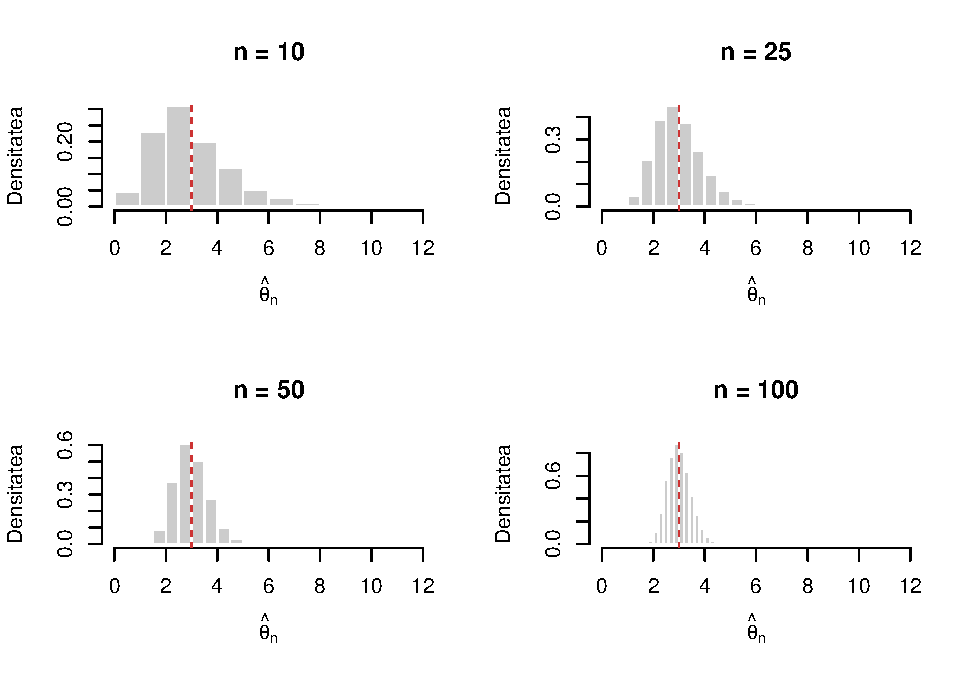
\includegraphics[width=0.7\linewidth]{Lab_6_files/figure-latex/unnamed-chunk-7-1} \end{center}

Ce se întâmplă dacă în loc de \(\hat{\theta}_n\) considerăm estimatorul
\(\tilde{\theta}_n = \bar{X}_n\) sau estimatorul
\(\dot{\theta}_n = \sqrt{\bar{X}_n S_n^2}\) ?

Pentru \(\tilde{\theta}_n\) avem

\begin{verbatim}
[1] "Pentru n = 10 varianta estimatorului este 0.301055748790976"
[1] "Pentru n = 25 varianta estimatorului este 0.118347691085662"
[1] "Pentru n = 50 varianta estimatorului este 0.0600801199663993"
[1] "Pentru n = 100 varianta estimatorului este 0.0296748320834817"
\end{verbatim}

\begin{center}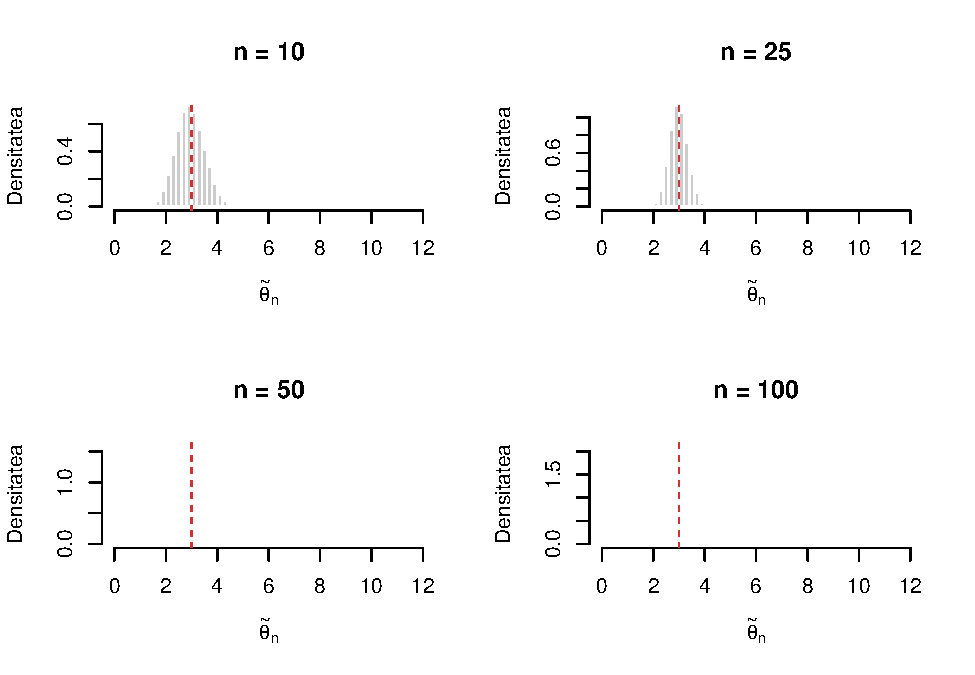
\includegraphics[width=0.7\linewidth]{Lab_6_files/figure-latex/unnamed-chunk-8-1} \end{center}

iar pentru \(\dot{\theta}_n\) avem

\begin{verbatim}
[1] "Pentru n = 10 varianta estimatorului este 0.771286077961343"
[1] "Pentru n = 25 varianta estimatorului este 0.305968043909498"
[1] "Pentru n = 50 varianta estimatorului este 0.151093564634052"
[1] "Pentru n = 100 varianta estimatorului este 0.075734675439954"
\end{verbatim}

\begin{center}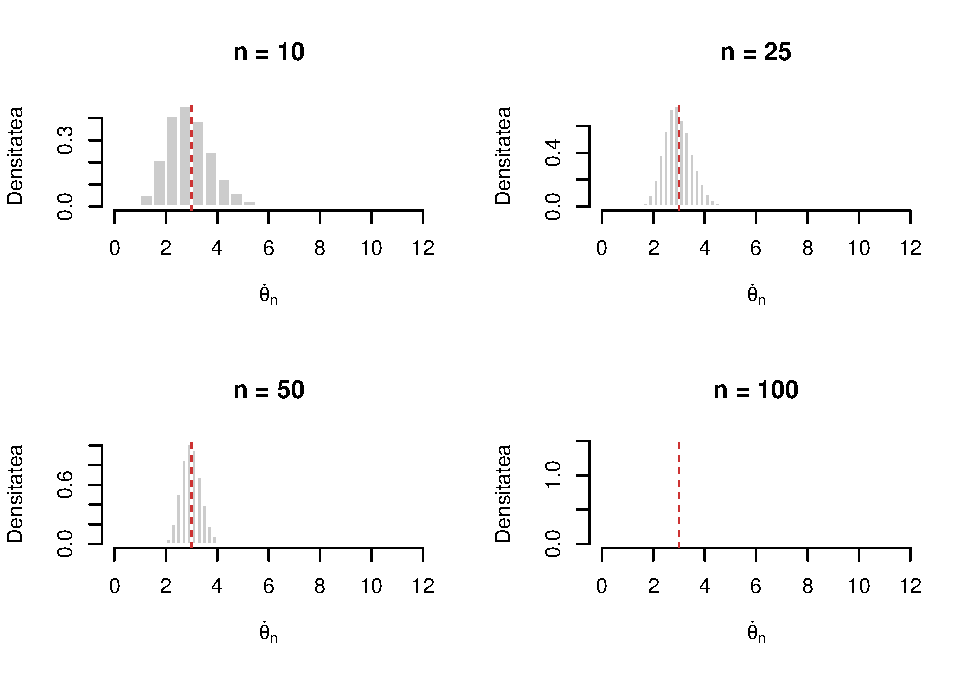
\includegraphics[width=0.7\linewidth]{Lab_6_files/figure-latex/unnamed-chunk-9-1} \end{center}


\end{document}
